\documentclass[spanish]{beamer}

\usepackage[es-tabla]{babel}
\usepackage{parskip}
\usepackage[capitalise, noabbrev]{cleveref}
\crefname{table}{\spanishtablename}{\spanishtablename}



\title{
	\textbf{
		Desarrollo de un modelo fundacional estocástico basado en procesos Gaussianos para la clasificación de bioseñales EEG en el diagnóstico asistido del TDAH.
	}
	}
\author{
	Julián David Pastrana Cortés, M.Sc.
	}


\date{}

\begin{document}
	
	
\frame{\titlepage}

\begin{frame}
	\frametitle{Motivation}
	\begin{figure}[htbp]
		\centering
		\begin{subfigure}[t]{0.48\textwidth}
			\centering
			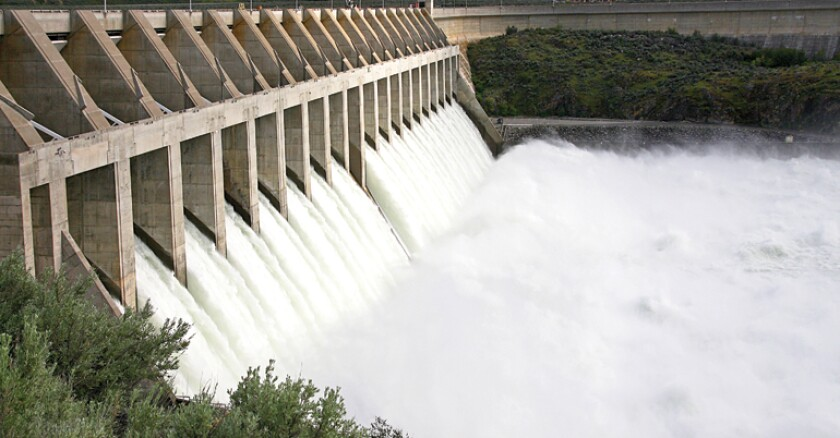
\includegraphics[width=\linewidth,height=2.7cm,keepaspectratio]{figures/hydro_gen.jpeg}
			\caption{Energy Generation}
		\end{subfigure}
		\hfill
		\begin{subfigure}[t]{0.48\textwidth}
			\centering
			
\includegraphics[width=\linewidth,height=2.7cm,keepaspectratio]{figures/stock_prices.jpg}
			\caption{Stock Prices}
		\end{subfigure}
		\\[1ex] % small vertical gap
		\begin{subfigure}[t]{0.48\textwidth}
			\centering
			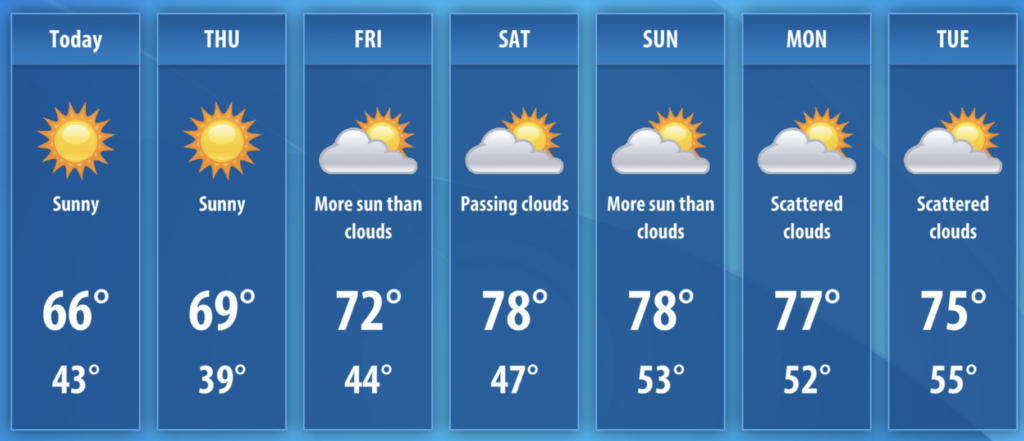
\includegraphics[width=\linewidth,height=2.7cm,keepaspectratio]{figures/weather_data.png}
			\caption{Weather Data}
		\end{subfigure}
	\end{figure}
	
	\begin{block}{\textbf{Challenges}}
		Non-linearities, high stochasticity, and complex patterns.
	\end{block}
	
\end{frame}

\begin{frame}{Point Estimation vs. Distribution Estimation}

\centering
\begin{tikzpicture}
	\begin{groupplot}[
		group style={
			group name=my plots,
			group size=2 by 1,
			horizontal sep=0.8cm,
		},
		width=5cm,
		height=4cm,
		scale only axis,
		axis lines=left,
		ymin=0, ymax=1,
		xmin=0, xmax=5.5, 
		]
		% Left subplot: Point Estimate Prediction
		\nextgroupplot[
		xlabel={Time},
		title={Point Estimation},
		yticklabel=\empty,
		]
		\addplot+[smooth, thick] coordinates {(0,0.2) (1,0.3) (2,0.5) (3,0.7) (4,0.8)};
		\addplot[only marks, mark=*, red] coordinates {(5,0.85)};
		
		% Right subplot: Distribution Estimation with Error Bars
		\nextgroupplot[
		xlabel={Time},
		title={Distribution Estimation},
		yticklabel=\empty,
		]
		\addplot+[smooth, thick] coordinates {(0,0.2) (1,0.3) (2,0.5) (3,0.7) (4,0.8)};
		
		% Define the right boundary of the predictive distribution at time=5
		\addplot[
		name path=right,
		domain=0.65:1.05,
		variable=\y,
		samples=100,
		draw=none,
		]
		({5 + 0.2*exp(-((\y-0.85)^2)/(2*0.004))}, {\y});
		
		% Define the left boundary of the predictive distribution at time=5
		\addplot[
		name path=left,
		domain=0.65:1.05,
		variable=\y,
		samples=100,
		draw=none,
		]
		({5 - 0.2*exp(-((\y-0.85)^2)/(2*0.004))}, {\y});
		
		% Fill between the two boundaries to show the uncertainty distribution
		\addplot[
		fill=red!20,
		fill opacity=0.5,
		draw=none,
		] fill between[of=right and left];
		
		% Mark the point prediction
		\addplot[only marks, mark=*, red] coordinates {(5,0.85)};
		
	\end{groupplot}
	
\end{tikzpicture}

\begin{block}{}
	Sometimes, a single point prediction is not enough. How confident is the model in its prediction?
\end{block}

\end{frame}

\begin{frame}{The Chained Correlated Gaussian Process Model}
	content...
\end{frame}
	
\end{document}